\documentclass[pdftex,a4paper,10pt,twoside,titlepage,italian]{article}
\usepackage[italian]{babel}
\usepackage[utf8]{inputenc}
\usepackage{fancyhdr,graphicx}
\usepackage[hmargin=2cm,vmargin=2cm,a4paper]{geometry}
\usepackage{hyperref}
\usepackage{xcolor}
\usepackage{multirow}
\pagestyle{fancy}
\lhead{\scshape Curriculum Vitae}
\rhead{\itshape Mauro Donadeo}
\rfoot{\footnotesize pag. \thepage}
\cfoot{}
\lfoot{{\footnotesize Aggiornato al: }\today}
\renewcommand{\headrulewidth}{.5pt}
\renewcommand{\footrulewidth}{.5pt}
%\renewcommand{\LettrineFontHook}{\color[gray]{0.5}}
%\renewcommand*\familydefault{\sfdefault}
\renewcommand*\labelitemi{$\textcolor{black!30}{\bullet}$}
%\definecolor{listings-comment-color}{RGB}{20,0,0}

\begin{document}
\begin{center}
\rule{.8 \textwidth}{1pt}\\[5pt]
\begin{minipage}{.55\textwidth}
	\LARGE\textbf{Mauro Donadeo}\\[16pt]
	\footnotesize{born 18th January 1986}\\
	\footnotesize Via Isonzo 136/7 \\ 
	35143 - Padova (PD)\\
	email: \texttt{mauro.donadeo@gmail.com}\\
	\footnotesize {no. Tel: +39 346 784 6243}\\
	\footnotesize Nationality: Italian\\
	\footnotesize {Skype: mauro.donadeo}
%	\footnotesize Stato civile: Celibe\\
\end{minipage}
\begin{minipage}{.25\textwidth}
	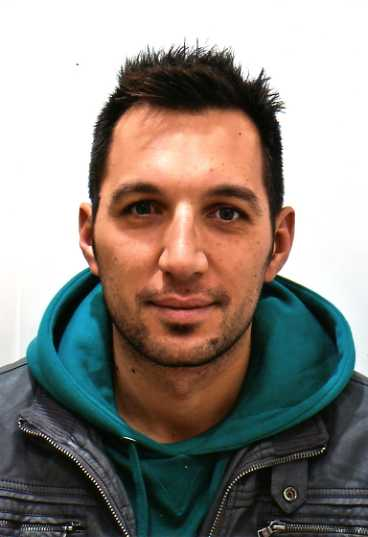
\includegraphics[width=\textwidth]{io.jpg}
\end{minipage}
\rule{.8 \textwidth}{1pt}\\[5pt]
\end{center}
\vspace{0.5cm}
\section*{Work Experience}
\begin{tabular}{l p{0.8\textwidth}}
July 2012 - Today & Research grant at University of Padua - DEI \\
& Creation of a library for  hand detection and hand gesture recognition.
Through acquisition images with low cost system (i.e. Microsoft Kinect). This system's developed in  
\textit{C++} with the library \textit{OpenCV, OpenNI, VTK, PCL e Qt}.\\
 & \\
January 2011 - June 2012 & Software engineer  in University of Padua - DPG.\\
& Developed a system of gesture recognize with images acquisited trough MS Kinect. System
developed in C++ with the library OpenCV and OpenNI. Visual feedback reproduced with \textit{Unity 3D}.
This project was developed in the European Project CEEDs (http//ceeds-project.eu).\\
November 2011 - December 2011 & Web designer for SimNumerica srl.\\
& Creating web page with CMS Drupal. Particular focus on: module login, news-slider, 
		trouble ticketing module and creating a wiki for administrator user.\\
September 2008 - August 2009 &  Computer assistant for certification courses office - SID (University of Padua)\\
& Comparing University's database of didactic area with Minister data.
 Web application to automate control student's didactic activity for generating the \textit{diploma supplement}.\\
 December 2007  -  August 2008 & Computer assistant in Technical and Network coordination office in Veneto Region\\
 & Design and implementation portal {\texttt overnetwork.it} based on \textit{CMS Joomla};
  focused on: creation system of trouble ticketing (with mail alert system) and new system of user's profiling. Participation in the project 802.1x.\\
 September 2005 - October 2007 & Postman various times and various towns in the province of Padua.
\end{tabular} 
\section*{Education}
\begin{itemize}
	\item Master Degree in Computer Engineering (University of Padova, October 2011).\\
	Thesis: {\itshape 3D Real time video conferencing system based on Microsoft Kinect sensor: design and implementation }
	\item Bachelor Degree in Computer Engineering (University of Padova, April 2008). \\Thesis:
	{\itshape Simulator in Java for the robotic system Lego NXT: design and implementation}
	\item High School Diploma, Computer Specialization (I.T.I.S. A. Meucci of Casarano (LE), 2004)
\end{itemize}

\section*{Computer skills}
\begin{itemize}
	\item \textbf{S.O.:} Gnu/Linux: Debian \& Acrhlinux from installation to configuration. Microsoft Windows XP and Microsoft Windows 7
	\item \textbf{Programming:} Java, C/C++ (also Microsoft Visual Studio 2010) and C\# (base) and for web programming experience: php, mySql
	\item \textbf{Other:} \LaTeX, OpenGL, vim, Matlab, Office, DirectX10, OpenNI,
	NXC,little work experience: Photoshop and Flash
\end{itemize}
\section*{Language skills}
\begin{itemize}
	\item \textbf{Italian:} native
	\item \textbf{English:} good skills in reading, writing and listening
	\item \textbf{Spanish:} good skills in reading, writing and listening (partecipated in a University foreign exchange program (Erasmus) in Barcelona from September 2009 to July 2010)
\end{itemize}
\section*{Personal Interests}
\begin{itemize}
	\item Editing video and images, computer science, mobile technology
	\item Hobbies: swimming, jogging, football, reading, travelling
\end{itemize}

\end{document}
